%%%%%%%%%%%%%%%%%%%%%%%%%%%%%%%%%%%%
% Slide options
%%%%%%%%%%%%%%%%%%%%%%%%%%%%%%%%%%%%

% Option 1: Slides with solutions

\documentclass[slidestop,compress,mathserif]{beamer}
\newcommand{\soln}[1]{\textit{#1}}
\newcommand{\solnGr}[1]{#1}

% Option 2: Handouts without solutions

%\documentclass[11pt,containsverbatim,handout]{beamer}
%\usepackage{pgfpages}
%\pgfpagesuselayout{4 on 1}[letterpaper,landscape,border shrink=5mm]
%\newcommand{\soln}[1]{ }
%\newcommand{\solnGr}{ }

%%%%%%%%%%%%%%%%%%%%%%%%%%%%%%%%%%%%
% Style
%%%%%%%%%%%%%%%%%%%%%%%%%%%%%%%%%%%%
\def\chp8@path{../../Chp 8}
\input{../../lec_style.tex}


%%%%%%%%%%%%%%%%%%%%%%%%%%%%%%%%%%%%
% Preamble
%%%%%%%%%%%%%%%%%%%%%%%%%%%%%%%%%%%%

\title[Lecture 32]{MA213: Lecture 32}
\subtitle{Module 5: Linear regression}
\author{OpenIntro Statistics, 4th Edition}
\institute{$\:$ \\ {\footnotesize Based on slides developed by Mine \c{C}etinkaya-Rundel of OpenIntro. \\
The slides may be copied, edited, and/or shared via the \webLink{http://creativecommons.org/licenses/by-sa/3.0/us/}{CC BY-SA license.} \\
Some images may be included under fair use guidelines (educational purposes).}}
\date{}


%%%%%%%%%%%%%%%%%%%%%%%%%%%%%%%%%%%%
% Begin document
%%%%%%%%%%%%%%%%%%%%%%%%%%%%%%%%%%%%

\begin{document}


%%%%%%%%%%%%%%%%%%%%%%%%%%%%%%%%%%%%
% Title page
%%%%%%%%%%%%%%%%%%%%%%%%%%%%%%%%%%%%

{
\addtocounter{framenumber}{-1} 
{\removepagenumbers 
\usebackgroundtemplate{\includegraphics[width=\paperwidth]{../../OpenIntro_Grid_4_3-01.jpg}}
\begin{frame}

\hfill \includegraphics[width=20mm]{../../oiLogo_highres}

\titlepage

\end{frame}
}
}


%%%%%%%%%%%%%%%%%%%%%%%%%%%%%%%%%%%%
% Recap/Agenda 
%%%%%%%%%%%%%%%%%%%%%%%%%%%%%%%%%%%%
% TODO better formatting
\begin{frame}
    \frametitle{Module 5: Linear regression}
    \begin{itemize}
        \item \hl{Previously: }Issues with Hypothesis Testing 2: Multiple comparisons
        \item \hl{This time: }Fitting a line, residuals, and correlation (Chapter 8.1)
        \item \hl{Reading: }Chapter 8.2 for next time
        \item \hl{Deadlines/Announcements: }HW 4.3 due today
    \end{itemize}
    
\end{frame}
%%%%%%%%%%%%%%%%%%%%%%%%%%%%%%%%%%%%
% Sections
%%%%%%%%%%%%%%%%%%%%%%%%%%%%%%%%%%%%

%%%%%%%%%%%%%%%%%%%%%%%%%%%%%%%%%%%%

\section{Review}

%%%%%%%%%%%%%%%%%%%%%%%%%%%%%%%%%%%%

\begin{frame}
    \frametitle{Last time: residuals and correlation}
\end{frame}

%%%%%%%%%%%%%%%%%%%%%%%%%%%%%%%%%%%%

\section{Fitting a line by least squares regression}

%%%%%%%%%%%%%%%%%%%%%%%%%%%%%%%%%%%%

\subsection{An objective measure for finding the best line}

%%%%%%%%%%%%%%%%%%%%%%%%%%%%%%%%%%%

\begin{frame}
\frametitle{An objective measure for finding the best line}

\begin{itemize}

\item We want a line that has small residuals:
\pause
\begin{enumerate}
\item Option 1: Minimize the sum of magnitudes (absolute values) of residuals
\[ |e_1| + |e_2| + \cdots + |e_n| \]
\pause
\item Option 2: Minimize the sum of squared residuals -- \hl{least squares}
\[ e_1^2 + e_2^2 + \cdots + e_n^2 \]
\end{enumerate}

\pause

\item Why least squares?
\pause
\begin{enumerate}
\item Most commonly used
\pause
\item Easier to compute by hand and using software
\pause
\item In many applications, a residual twice as large as another is usually more than twice as bad
\end{enumerate}

\end{itemize}

\end{frame}

%%%%%%%%%%%%%%%%%%%%%%%%%%%%%%%%%%

\begin{frame}
\frametitle{The least squares line}

\[ \mathhl{ \hat{y} = \beta_0 + \beta_1 x } \]

\begin{itemize}
\item $\hat{y}$: Predicted value of the response variable, $y$
\item $\beta_0$: Intercept, parameter
\begin{itemize}
\item $b_0$: Intercept, point estimate
\end{itemize}
\item $\beta_1$: Slope, parameter
\begin{itemize}
\item $b_1$: Slope, point estimate
\end{itemize}
\item $x$: Explanatory variable
\end{itemize}

\end{frame}

%%%%%%%%%%%%%%%%%%%%%%%%%%%%%%%%%%

\subsection{Conditions for the least squares line}

%%%%%%%%%%%%%%%%%%%%%%%%%%%%%%%%%%%

\begin{frame}
\frametitle{Conditions for the least squares line}

\begin{enumerate}

\item Linearity

\pause

\item Nearly normal residuals

\pause

\item Constant variability

\end{enumerate}

\end{frame}

%%%%%%%%%%%%%%%%%%%%%%%%%%%%%%%%%%

\begin{frame}
\frametitle{Conditions: (1) Linearity}

\begin{itemize}

\item The relationship between the explanatory and the response variable should be linear. 

\pause

\item Methods for fitting a model to non-linear relationships exist, but are beyond the scope of this class. If this topic is of interest, an \href{http://www.openintro.org/download.php?file=os2_extra_nonlinear_relationships&referrer=/stat/textbook.php}{Online Extra is available on openintro.org} covering new techniques.

\pause

\item Check using a scatterplot of the data, or a \hl{residuals plot}.

\end{itemize}

\begin{center}
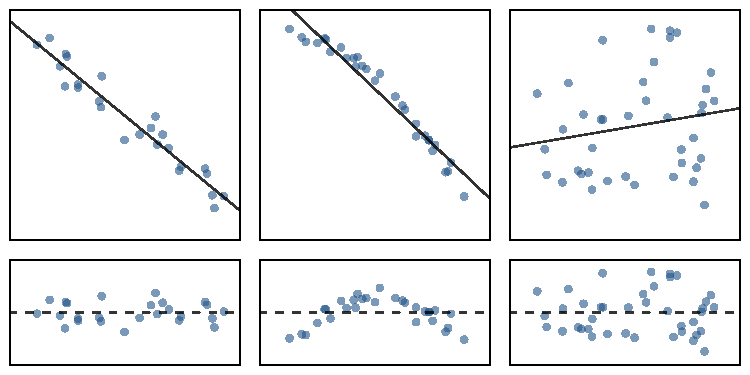
\includegraphics[width=0.7\textwidth]{\chp8@path/8-2_least_square_reg/figures/sampleLinesAndResPlots/sampleLinesAndResPlots}
\end{center}

\end{frame}

%%%%%%%%%%%%%%%%%%%%%%%%%%%%%%%%%%

\section{Edfinity Quiz: Checking the conditions}

%%%%%%%%%%%%%%%%%%%%%%%%%%%%%%%%%%

\section{R Demonstration: Slope and intercept}

%%%%%%%%%%%%%%%%%%%%%%%%%%%%%%%%%%

\section{Edfinity Quiz: Practice with slope and intercept}

%%%%%%%%%%%%%%%%%%%%%%%%%%%%%%%%%%

\section{R Demonstration: Regression, extrapolation}

%%%%%%%%%%%%%%%%%%%%%%%%%%%%%%%%%%

\section{Edfinity Quiz: Putting it all together}

%%%%%%%%%%%%%%%%%%%%%%%%%%%%%%%%%%

\begin{frame}
\frametitle{Anatomy of a residuals plot}

\twocol{0.5}{0.5}
{
\begin{center}
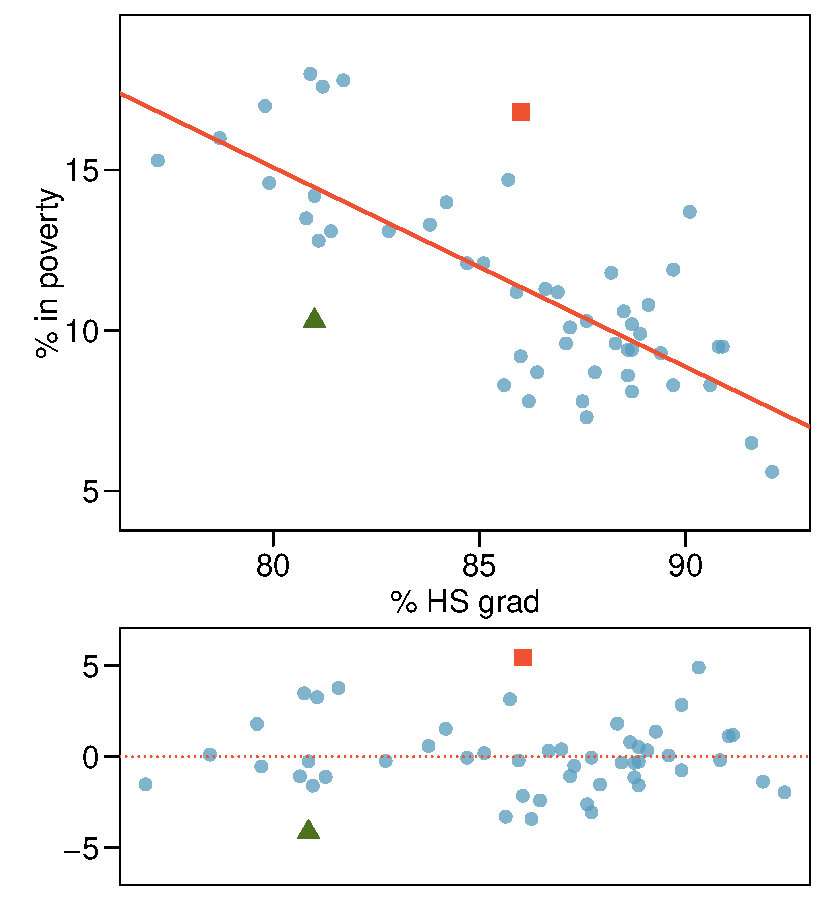
\includegraphics[width=\textwidth]{\chp8@path/8-2_least_square_reg/figures/poverty/poverty_hsgrad_resplot}
\end{center}
}
{
\green{{\LARGE $\blacktriangle$}} \hl{RI:}
\begin{align*}
\%~HS~grad &= 81 \qquad \%~in~poverty = 10.3 \\
\widehat{\%~in~poverty} &= 64.68 - 0.62 * 81 = 14.46 \\
e &= \%~in~poverty - \widehat{\%~in~poverty} \\
&= 10.3 - 14.46 = \green{$-4.16$}
\end{align*}
$\:$
\pause
\textcolor{red}{{\Large $\blacksquare$}} \hl{DC:}
\begin{align*}
\%~HS~grad &= 86 \qquad \%~in~poverty = 16.8 \\
\widehat{\%~in~poverty} &= 64.68 - 0.62 * 86 = 11.36 \\
e &= \%~in~poverty - \widehat{\%~in~poverty} \\
&= 16.8 - 11.36 = \textcolor{red}{5.44}
\end{align*}
}

\end{frame}


%%%%%%%%%%%%%%%%%%%%%%%%%%%%%%%%%%

\begin{frame}
\frametitle{Conditions: (2) Nearly normal residuals}

\begin{itemize}

\item The residuals should be nearly normal.

\pause

\item This condition may not be satisfied when there are unusual observations that don't follow the trend of the rest of the data.

\pause

\item Check using a histogram.

\end{itemize}

\begin{center}
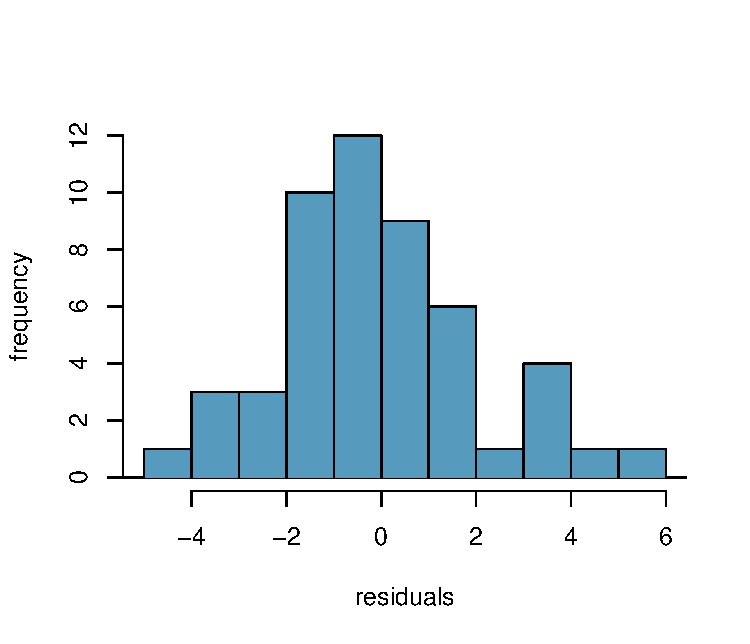
\includegraphics[width=0.5\textwidth]{\chp8@path/8-2_least_square_reg/figures/poverty/normal_res}
\end{center}

\end{frame}

%%%%%%%%%%%%%%%%%%%%%%%%%%%%%%%%%%

\begin{frame}
\frametitle{Conditions: (3) Constant variability}

\twocol{0.5}{0.5}
{
\begin{center}
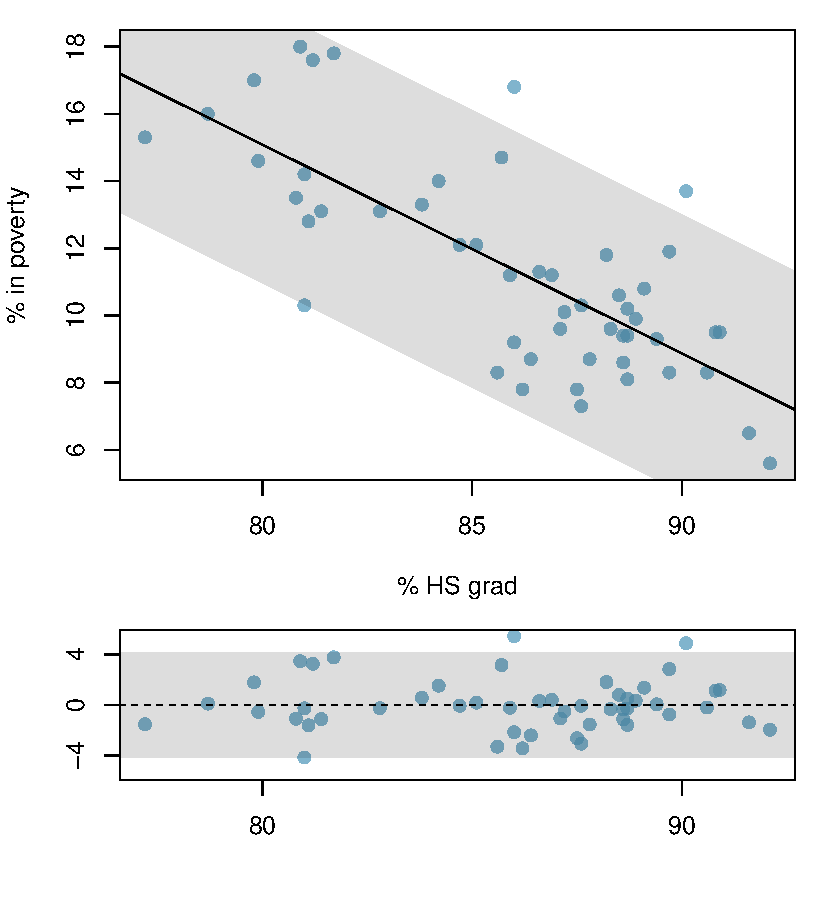
\includegraphics[width=\textwidth]{\chp8@path/8-2_least_square_reg/figures/poverty/poverty_hsgrad_tube}
\end{center}
}
{
\begin{itemize}

\item The variability of points around the least squares line should be roughly constant.

\pause

\item This implies that the variability of residuals around the 0 line should be roughly constant as well.

\pause

\item Also called \hl{homoscedasticity}.

\pause

\item Check using a residuals plot.

\end{itemize}
}


\end{frame}

%%%%%%%%%%%%%%%%%%%%%%%%%%%%%%%%%%

\begin{frame}
\frametitle{Checking conditions}

\twocol{0.5}{0.5}
{
\pq{What condition is this linear model obviously violating?}
\begin{enumerate}[(a)]
\item Constant variability
\solnMult{Linear relationship}
\item Normal residuals
\item No extreme outliers
\end{enumerate}
}
{
\begin{center}
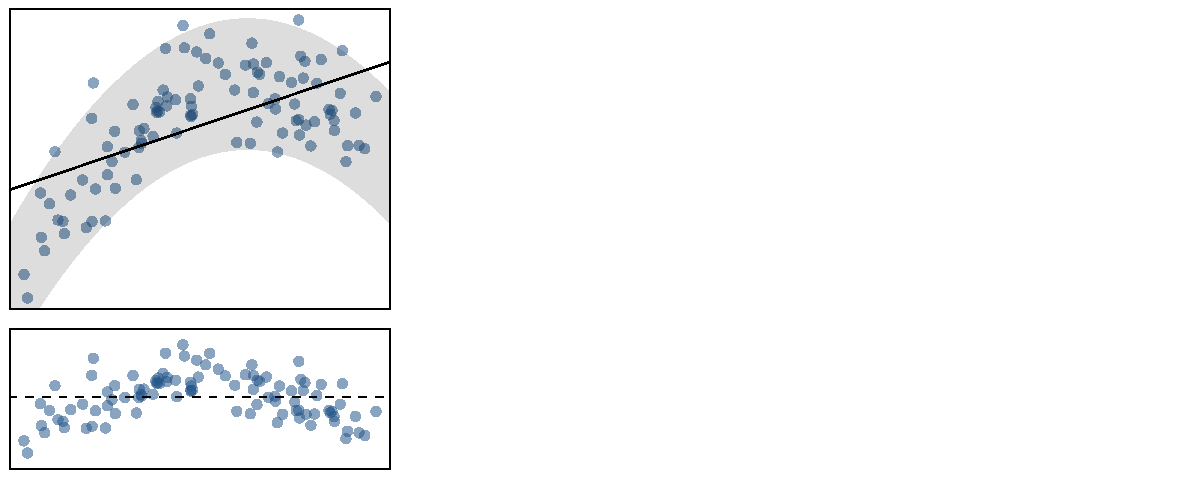
\includegraphics[width=\textwidth]{\chp8@path/8-2_least_square_reg/figures/problems/nonlinear}
\end{center}
}

\end{frame}

%%%%%%%%%%%%%%%%%%%%%%%%%%%%%%%%%%

\begin{frame}
\frametitle{Checking conditions}

\twocol{0.5}{0.5}
{
\pq{What condition is this linear model obviously violating?}
\begin{enumerate}[(a)]
\solnMult{ Constant variability}
\item Linear relationship
\item Normal residuals
\item No extreme outliers
\end{enumerate}
}
{
\begin{center}
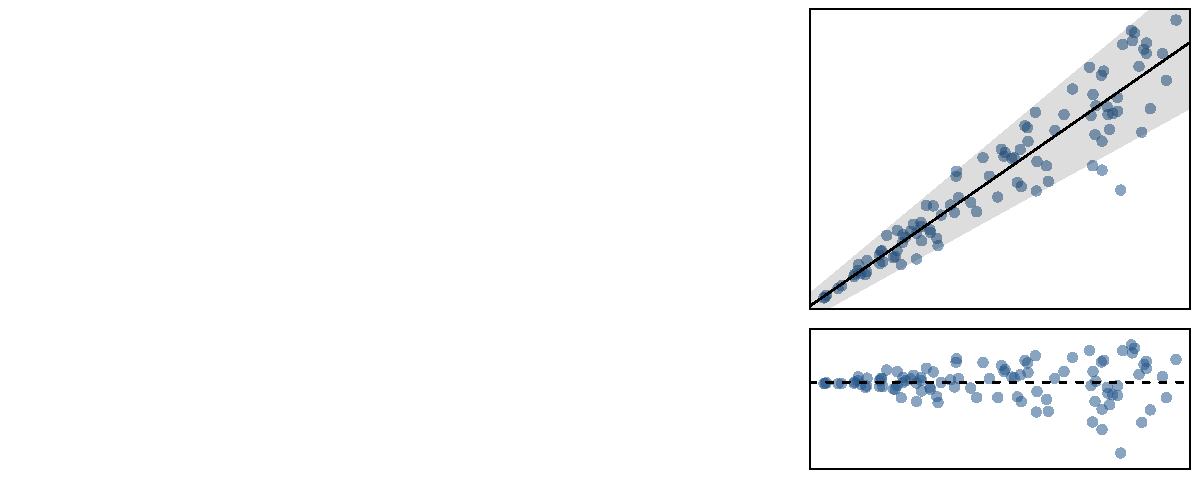
\includegraphics[width=\textwidth]{\chp8@path/8-2_least_square_reg/figures/problems/heteroscedastic}
\end{center}
}

\end{frame}

%%%%%%%%%%%%%%%%%%%%%%%%%%%%%%%%%%%

\subsection{Finding the least squares line}

%%%%%%%%%%%%%%%%%%%%%%%%%%%%%%%%%%%

\begin{frame}
\frametitle{Given...}

\twocol{0.5}{0.5}
{
\begin{center}
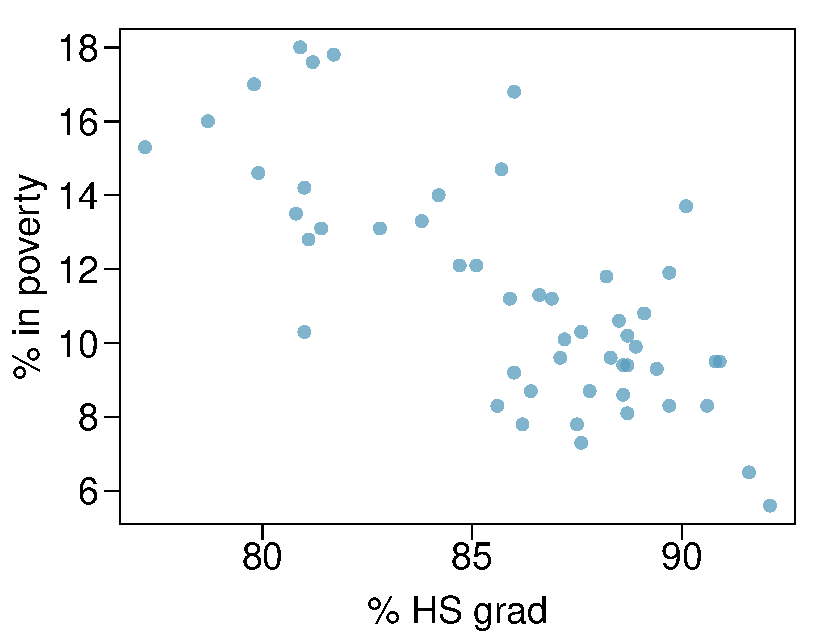
\includegraphics[width=\textwidth]{\chp8@path/8-2_least_square_reg/figures/poverty/poverty_hsgrad}
\end{center}
}
{
\begin{tabular}{l r r}
\hline
		& \% HS grad		& \% in poverty \\
		& $(x)$			& $(y)$ \\
\hline
mean	& $\bar{x} = 86.01$	& $\bar{y} = 11.35$  \\
sd		& $s_x = 3.73$		& $s_y = 3.1$ \\
\hline
		& correlation		& $R = -0.75$ \\
\hline
\end{tabular}
}

\end{frame}

%%%%%%%%%%%%%%%%%%%%%%%%%%%%%%%%%%

\subsection{Interpreting regression model parameter estimates}

%%%%%%%%%%%%%%%%%%%%%%%%%%%%%%%%%%

\begin{frame}
\frametitle{Slope}

\formula{Slope}
{The slope of the regression can be calculated as 
\[ b_1 = \frac{s_y}{s_x} R \]
}

\pause

\hl{In context...}
\[ b_1 = \frac{3.1}{3.73} \times -0.75 = -0.62 \]

\pause
$\:$ \\
\hl{Interpretation} \\
For each additional \% point in HS graduate rate, we would expect the \% living in poverty to be lower on average by 0.62\% points.

\end{frame}

%%%%%%%%%%%%%%%%%%%%%%%%%%%%%%%%%%

\begin{frame}
\frametitle{Intercept}

\formula{Intercept}
{The intercept is where the regression line intersects the $y$-axis. The calculation of the intercept uses the fact the a regression line always passes through $(\bar{x},\bar{y})$.
\[ b_0 = \bar{y} - b_1 \bar{x} \]
}

\pause

\twocol{0.68}{0.32}
{
\begin{center}
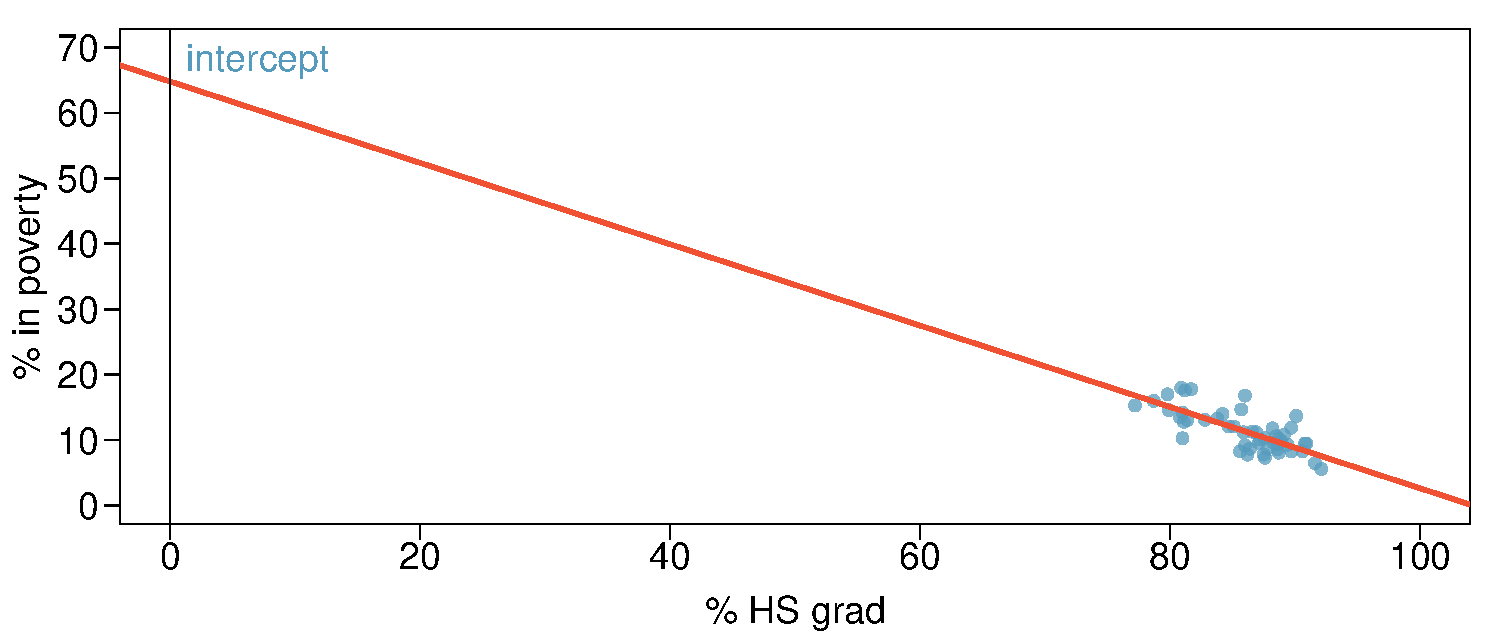
\includegraphics[width=\textwidth]{\chp8@path/8-2_least_square_reg/figures/poverty/poverty_hsgrad_line_wide}
\end{center}
}
{
\pause
\begin{align*}
b_0 &= 11.35 - (-0.62) \times 86.01 \\
&= 64.68
\end{align*}
}

\end{frame}

%%%%%%%%%%%%%%%%%%%%%%%%%%%%%%%%%%

\begin{frame}
\frametitle{}

\pq{Which of the following is the correct interpretation of the intercept?}

\begin{enumerate}[(a)]
\item For each \% point increase in HS graduate rate, \% living in poverty is expected to increase on average by 64.68\%.
\item For each \% point decrease in HS graduate rate, \% living in poverty is expected to increase on average by 64.68\%.
\item Having no HS graduates leads to 64.68\% of residents living below the poverty line.
\solnMult{States with no HS graduates are expected on average to have 64.68\% of residents living below the poverty line.}
\item In states with no HS graduates \% living in poverty is expected to increase on average by 64.68\%.
\end{enumerate}

\end{frame}

%%%%%%%%%%%%%%%%%%%%%%%%%%%%%%%%%%%

\begin{frame}
\frametitle{More on the intercept}

Since there are no states in the dataset with no HS graduates, the intercept is of no interest, not very useful, and also not reliable since the predicted value of the intercept is so far from the bulk of the data.

\begin{center}
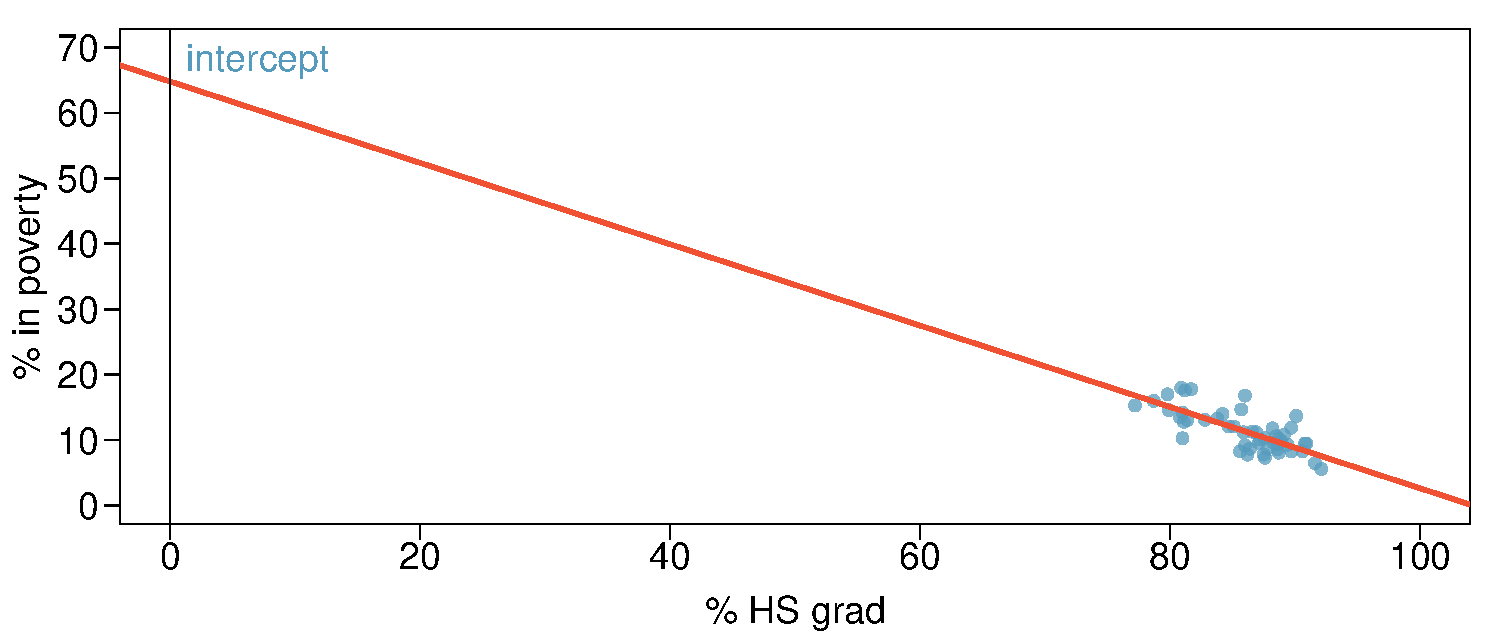
\includegraphics[width=\textwidth]{\chp8@path/8-2_least_square_reg/figures/poverty/poverty_hsgrad_line_wide}
\end{center}

\end{frame}

%%%%%%%%%%%%%%%%%%%%%%%%%%%%%%%%%%

\begin{frame}
\frametitle{Regression line}

\[ \widehat{\%~in~poverty} = 64.68 - 0.62~\%~HS~grad \]

\begin{center}
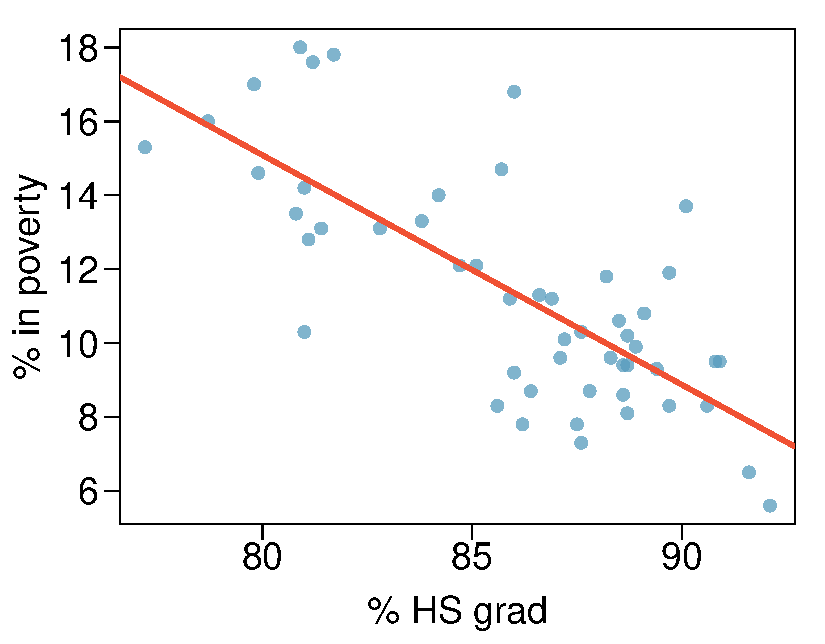
\includegraphics[width=0.7\textwidth]{\chp8@path/8-2_least_square_reg/figures/poverty/poverty_hsgrad_line}
\end{center}

\end{frame}

%%%%%%%%%%%%%%%%%%%%%%%%%%%%%%%%%%

\subsection{Recap: Interpreting the slope and the intercept}

%%%%%%%%%%%%%%%%%%%%%%%%%%%%%%%%%%%

\begin{frame}
\frametitle{Interpretation of slope and intercept}

\twocol{0.5}{0.5}{
\begin{itemize}

\item \hl{Intercept:} When {$x = 0$}, {$y$} is expected to equal {the intercept}. \\

$\:$ \\

\item \hl{Slope:} For each {unit} in {$x$}, {$y$} is expected to {increase / decrease} on average by {the slope}.

\end{itemize}
}
{
\begin{center}
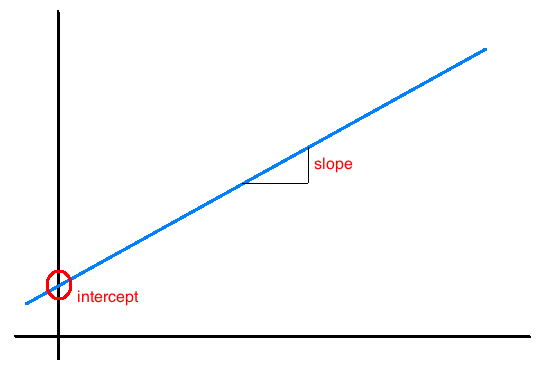
\includegraphics[width=\textwidth]{\chp8@path/8-2_least_square_reg/figures/diagram}
\end{center}
}

\vspace{1cm}

\Note{These statements are not causal, unless the study is a randomized controlled experiment.}

\end{frame}


%%%%%%%%%%%%%%%%%%%%%%%%%%%%%%%%%%

\subsection{Prediction \& extrapolation}

%%%%%%%%%%%%%%%%%%%%%%%%%%%%%%%%%%


\begin{frame}
\frametitle{Prediction}

\begin{itemize}

\item Using the linear model to predict the value of the response variable for a given value of the explanatory variable is called \hl{prediction}, simply by plugging in the value of $x$ in the linear model equation.

\item There will be some uncertainty associated with the predicted value.

\end{itemize}

\begin{center}
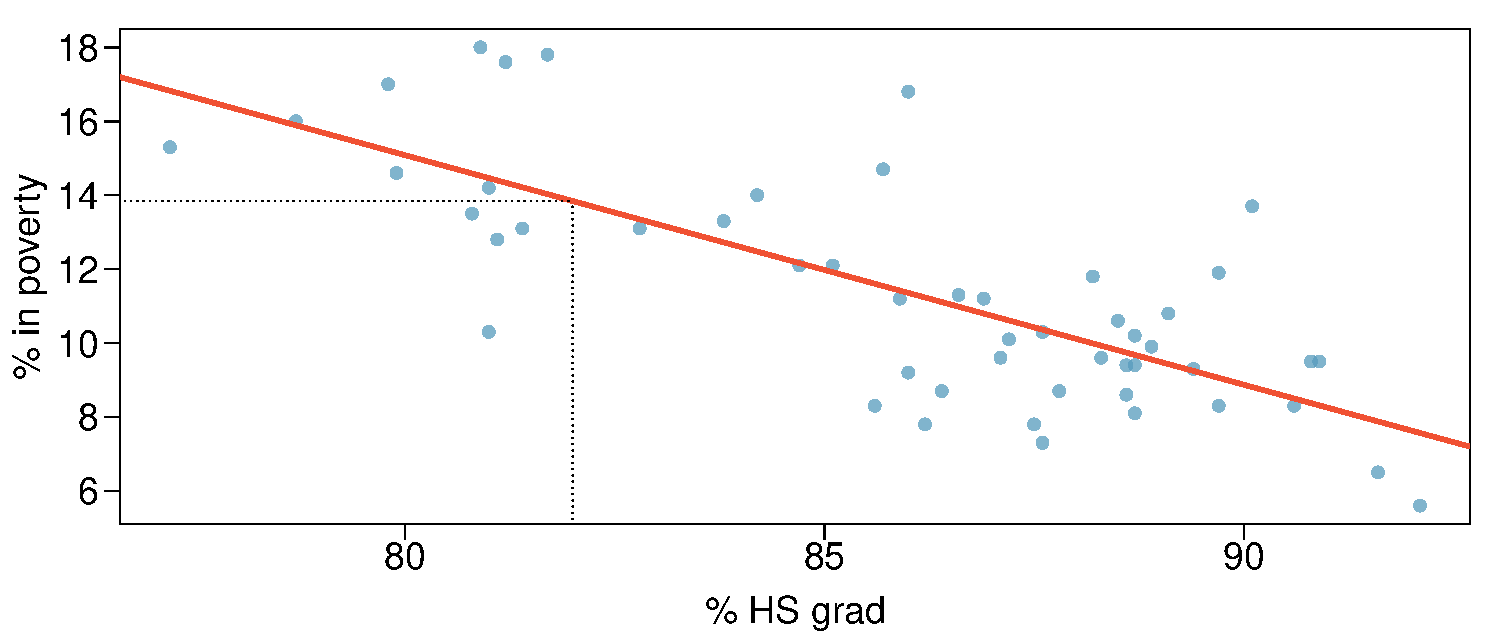
\includegraphics[width=0.9\textwidth]{\chp8@path/8-2_least_square_reg/figures/poverty/poverty_hsgrad_pred}
\end{center}

\end{frame}

%%%%%%%%%%%%%%%%%%%%%%%%%%%%%%%%%%

\begin{frame}
\frametitle{Extrapolation}

\begin{itemize}

\item Applying a model estimate to values outside of the realm of the original data is called \hl{extrapolation}.

\item Sometimes the intercept might be an extrapolation.

\end{itemize}

\begin{center}
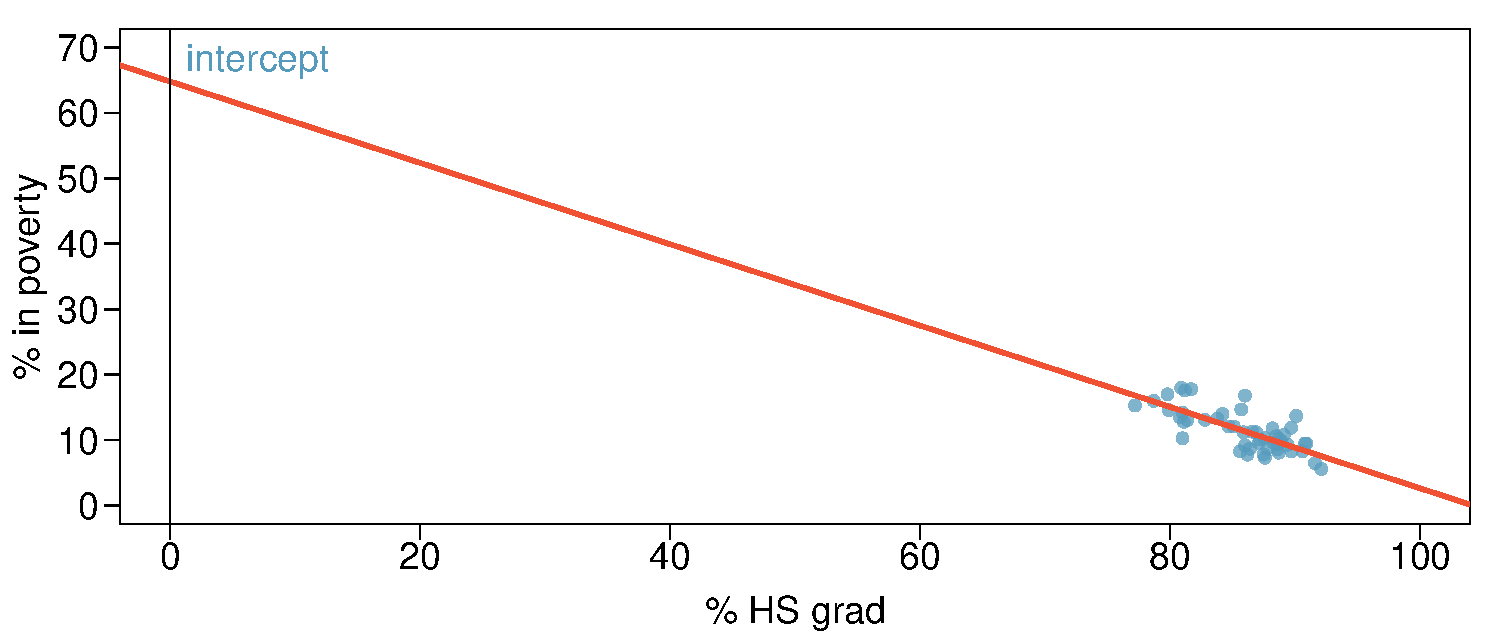
\includegraphics[width=\textwidth]{\chp8@path/8-2_least_square_reg/figures/poverty/poverty_hsgrad_line_wide}
\end{center}

\end{frame}

%%%%%%%%%%%%%%%%%%%%%%%%%%%%%%%%%%

\begin{frame}
\frametitle{Examples of extrapolation}

\begin{center}
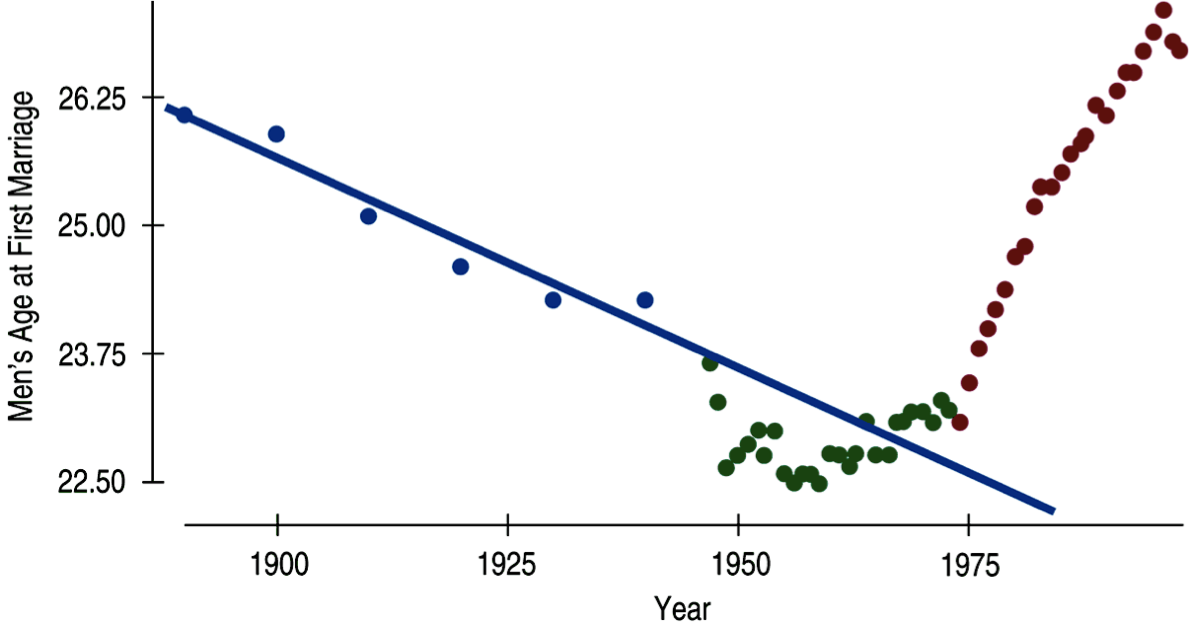
\includegraphics[width=\textwidth]{\chp8@path/8-2_least_square_reg/figures/extrapolation}
\end{center}

\end{frame}

%%%%%%%%%%%%%%%%%%%%%%%%%%%%%%%%%%

\begin{frame}
\frametitle{Examples of extrapolation}

\begin{center}
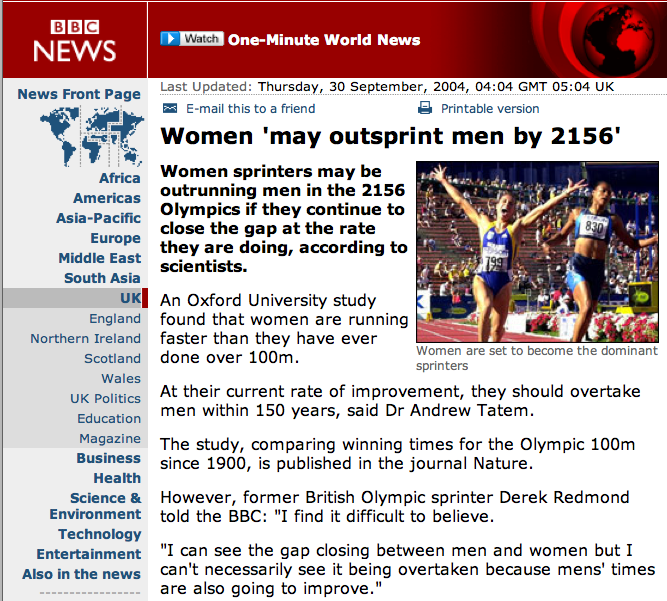
\includegraphics[width=0.7\textwidth]{\chp8@path/8-2_least_square_reg/figures/womenOutsprintBBC}
\end{center}

\end{frame}

%%%%%%%%%%%%%%%%%%%%%%%%%%%%%%%%%%

\begin{frame}
\frametitle{Examples of extrapolation}

\begin{center}
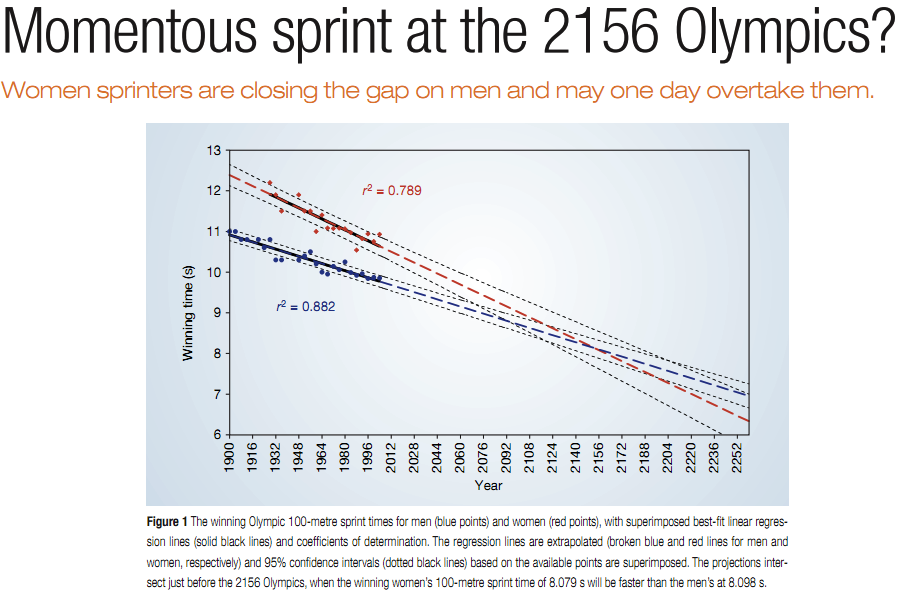
\includegraphics[width=\textwidth]{\chp8@path/8-2_least_square_reg/figures/womenOutsprint}
\end{center}

\end{frame}

%%%%%%%%%%%%%%%%%%%%%%%%%%%%%%%%%%

\subsection{Using $R^2$ to describe the strength of a fit}

%%%%%%%%%%%%%%%%%%%%%%%%%%%%%%%%%%%

\begin{frame}
\frametitle{$R^2$}

\begin{itemize}

\item The strength of the fit of a linear model is most commonly evaluated using \mathhl{R^2}.

\pause

\item $R^2$ is calculated as the square of the correlation coefficient.

\pause

\item It tells us what percent of variability in the response variable is explained by the model.

\pause

\item The remainder of the variability is explained by variables not included in the model or by inherent randomness in the data.

\pause

\item For the model we've been working with, $R^2 = (-0.75)^2 = 0.56$.

\end{itemize}

\end{frame}

%%%%%%%%%%%%%%%%%%%%%%%%%%%%%%%%%%

\begin{frame}
\frametitle{Interpretation of $R^2$}

\pq{{\small Which of the below is the correct interpretation of $R = -0.75$, $R^2 = 0.56$?}}

\twocol{0.65}{0.35}{
\begin{enumerate}[(a)]

\item 56\% of the variability in the \% of HG graduates among the 51 states is explained by the model.

\solnMult{ 56\% of the variability in the \% of residents living in poverty among the 51 states is explained by the model.}

\item 56\% of the time \% HS graduates predict \% living in poverty correctly.

\item 75\% of the variability in the \% of residents living in poverty among the 51 states is explained by the model.

\end{enumerate}
}{
\begin{center}
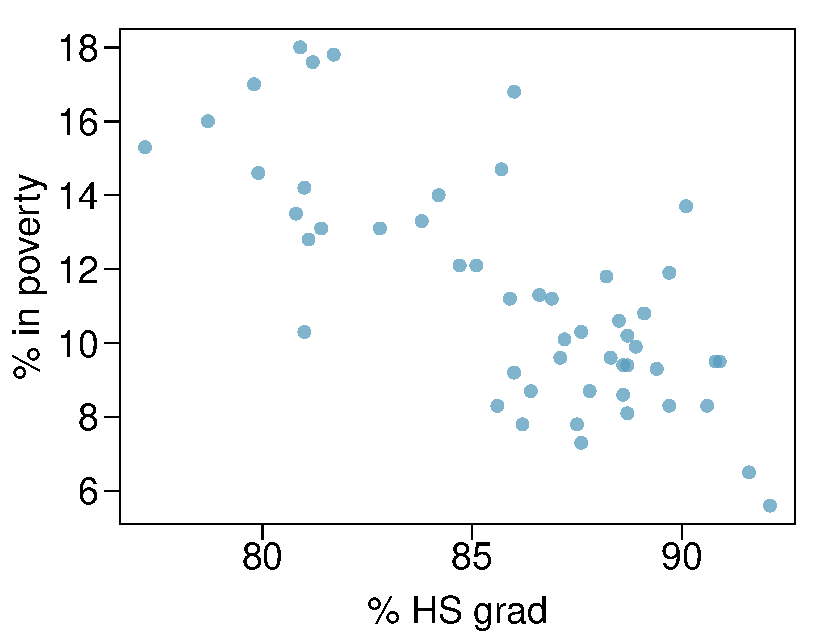
\includegraphics[width=\textwidth]{\chp8@path/8-2_least_square_reg/figures/poverty/poverty_hsgrad}
\end{center}
}

\end{frame}

%%%%%%%%%%%%%%%%%%%%%%%%%%%%%%%%%%


%%%%%%%%%%%%%%%%%%%%%%%%%%%%%%%%%%%%
% End document
%%%%%%%%%%%%%%%%%%%%%%%%%%%%%%%%%%%%

\end{document}